% document class and packages
\documentclass{beamer}
%\usepackage{adjustbox}
%\usepackage{algorithm,algorithmic}
%\usepackage{amsmath}
%\usepackage{amssymb}
%\usepackage{graphicx}
%\usepackage{hyperref}
\usepackage{color}
\usepackage{pgfplots}
\pgfplotsset{compat=newest}
\usetikzlibrary{arrows,decorations.markings}

\tikzset{myptr/.style={decoration={markings,mark=at position 1 with %
    {\arrow[scale=1.5,>=stealth]{>}}},postaction={decorate}}}

% indent for algorithm pseudo-code
\newlength\myindent
\setlength\myindent{1em}
\newcommand\bindent{%
  \begingroup
  \setlength{\itemindent}{\myindent}
  \addtolength{\algorithmicindent}{\myindent}
}
\newcommand\eindent{\endgroup}

% remove figure caption prefix
\setbeamertemplate{caption}{\raggedright\insertcaption\par}

% hyperlinks setup
\hypersetup{colorlinks,breaklinks,
	urlcolor=[rgb]{0,0.75,1},
	linkcolor=[rgb]{0.75,0.75,0.75}}

% empty navigation symbols
\beamertemplatenavigationsymbolsempty

% remove navigation dots on miniframes
\makeatletter
\def\beamer@writeslidentry{\clearpage\beamer@notesactions}
\makeatother

% Use Theme
\usetheme{Warsaw}
\useoutertheme[footline=authortitle]{miniframes}
\useinnertheme[shadow=true]{rounded}

% Colors
\definecolor{black}{RGB}{0,0,0} % black
\definecolor{dgreen}{RGB}{0,73,73} % dark green
\definecolor{lgreen}{RGB}{0,146,146} % light green
\definecolor{dpink}{RGB}{255,109,182} % dark pink
\definecolor{lpink}{RGB}{255,182,119} % light pink
\definecolor{dpurple}{RGB}{73,0,146} % dark purple
\definecolor{dblue}{RGB}{0,109,219} % dark blue
\definecolor{lpurple}{RGB}{182,109,255} % light purple
\definecolor{lblue}{RGB}{109,182,255} % light blue
\definecolor{pblue}{RGB}{182,219,255} % powder blue
\definecolor{dred}{RGB}{146,0,0} % dark red
\definecolor{brown}{RGB}{146,73,0} % brown
\definecolor{orange}{RGB}{219,209,0} % orange
\definecolor{bgreen}{RGB}{36,255,36} % bright green
\definecolor{yellow}{RGB}{255,255,109} % yellow

% New Commands
\newcommand\proj[2]{\textrm{proj}_{\textbf{#2}}{\textbf{#1}}}
\newcommand\abs[1]{\left|#1\right|}
\newcommand\norm[1]{\left\Vert#1\right\Vert}
\newcommand\vv[2]{\left\langle #1,#2\right\rangle}
\newcommand\vvv[3]{\left\langle #1,#2,#3\right\rangle}

% Beamer Colors
\setbeamercolor{palette primary}{bg=black,fg=black!10}
\setbeamercolor{palette secondary}{bg=lblue,fg=black!10}
\setbeamercolor{palette tertiary}{bg=black,fg=black!10}
\setbeamercolor{structure}{fg=black}
\setbeamercolor{frametitle}{fg=black}

% Title Page
\title{Sinquefield Cup}
\author{Thomas R. Cameron}
\institute{Davidson College}
\date{\today}

\begin{document}
% Title Frame
\begin{frame}
	\titlepage
\end{frame}

\begin{frame}{Round by Round Analysis}
\centering
\resizebox{0.80\textwidth}{!}{% Sinquefield Cup
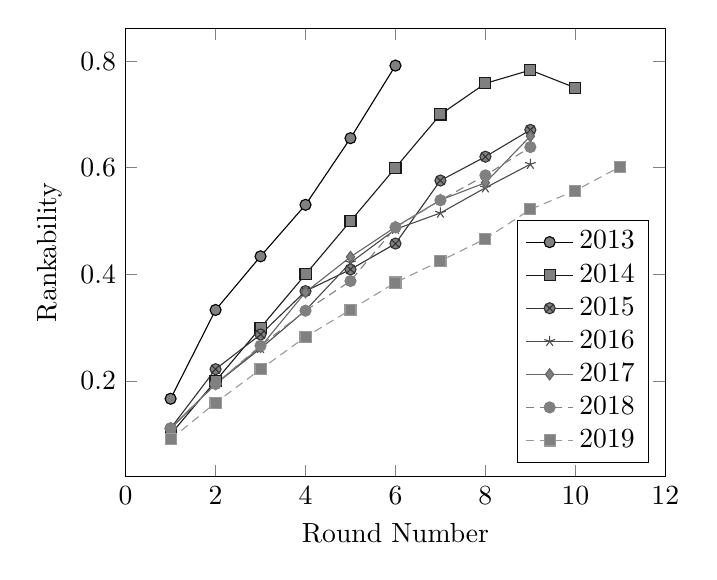
\begin{tikzpicture}
	\begin{axis}[
		xlabel = Round Number,
		ylabel =  Rankability,
		legend pos = south east,
		cycle list name = black white]
		\addplot+[black] coordinates{
			(1,0.1667)
			(2,0.3333)
			(3,0.4339)
			(4,0.5305)
			(5,0.6555)
			(6,0.7917)
		};
		\addplot+[black!90] coordinates{
			(1,0.1000)
			(2,0.2000)
			(3,0.3000)
			(4,0.4000)
			(5,0.5000)
			(6,0.6000)
			(7,0.7000)
			(8,0.7583)
			(9,0.7832)
			(10,0.7500)
		};
		\addplot+[black!80] coordinates{
			(1,0.1111)
			(2,0.2222)
			(3,0.2873)
			(4,0.3686)
			(5,0.4093)
			(6,0.4578)
			(7,0.5761)
			(8,0.6208)
			(9,0.6711)
		};
		\addplot+[black!70] coordinates{
			(1,0.1111)
			(2,0.1944)
			(3,0.2611)
			(4,0.3325)
			(5,0.4220)
			(6,0.4846)
			(7,0.5152)
			(8,0.5625)
			(9,0.6067)
		};
		\addplot+[black!60] coordinates{
			(1,0.1111)
			(2,0.1944)
			(3,0.2639)
			(4,0.3666)
			(5,0.4328)
			(6,0.4889)
			(7,0.5395)
			(8,0.5719)
			(9,0.6593)
		};
		\addplot+[black!50] coordinates{
			(1,0.1111)
			(2,0.1944)
			(3,0.2662)
			(4,0.3319)
			(5,0.3876)
			(6,0.4882)
			(7,0.5391)
			(8,0.5857)
			(9,0.6389)
		};
		\addplot+[black!40] coordinates{
			(1,0.0909)
			(2,0.1591)
			(3,0.2220)
			(4,0.2826)
			(5,0.3336)
			(6,0.3847)
			(7,0.4252)
			(8,0.4668)
			(9,0.5219)
			(10,0.5572)
			(11,0.6021)
		};
		\legend{2013, 2014, 2015, 2016, 2017, 2018,2019}
	\end{axis}
\end{tikzpicture}%
}
\end{frame}

\end{document}